\section{Tests}\label{sec: tests}

The \texttt{python} folder contains scripts to calibrate, test, evaluate, and compare calibrations. 
%
Table \ref{tab: python scripts} presents a summary of the scripts found in the folder. 

\begin{table}[h]
	\centering
	\caption{Brief description of the python scripts.}
	\label{tab: python scripts}
	\begin{tabulary}{\linewidth}{C|L}
		\toprule
		Script & Description \\\midrule
		applyCalib.py & Performs the calibration over a set of calibration data using different combinations of the options described in Section \ref{subsec: options}. \\\hline
		checkStaticData.py & Reads a set of data collected with the static camera in different orientations and plots the gyroscope readings distributions. This allows an visualisation of the gyroscope bias according to its orientation (i.e. depending on the accelerometer readings).\\\hline
		madgwickahrs.py & Madgwick filter used to remove the gravity from the accelerometer for the integration tests. \\\hline
		plotCalibBiasAndIntegration.py & Reads the calibration parameter for each calibration data and each calibration option, calculates the calibrated values for the accelerometer and gyroscope readings for a set of test data, and visualise the resulting magnitude of the accelerometer and gyroscope biases.
		
		It also performs and visualises the integration tests, in which the orientation and linear velocities are calculated from the gyroscope and accelerometer, respectively, given a metric for the impact of the calibration.\\\hline
		
		quaternion.py & Basic library for handling quaternions. Useb by the Madgwick filter.\\\hline
		utils.py & Miscellaneous functions used by the other scripts. \\\hline
		test.py & Development board. do not use.\\
		\bottomrule
	\end{tabulary}
\end{table}

\subsection{Integration Tests}\label{subsec: integration tests}

The calibrations evaluation is two-fold. 
%
On one hand we perform several calibrations, with the same options, and evaluate which one gives the best results.
%
On the other hand, we want to perform calibrations with different options, and evaluate which ones lead to the best results.
%
Regardless, we test it over several test data, to have an idea of the overall precision.
%
We collected $10$ calibration data, using $5$ combinations of calibration options, and tested over $10$ test data, givin a total of $500$ tests.

As a metric we perform a simple integration of the accelerometer into the linear velocities, and from the gyroscope into orientation.
%
The test data always start and ends with the stationary camera, and the initial and final orientation is approximately the same, which is obtained by aligning tow surfaces of the IMU box with two flat surfaces (wall and table).

Before calculating the linear velocities, the gravity effect on the accelerometer is removed using the Madgwick filter. 
%
And the first $20~s$ of the  data is discarded, giving time for the Madgwick filter convergence, during this period the camera was stationary.

Figure \ref{fig:comparecalibrationtrials} shows the comparison between calibration trials, showing that the accelerometer calibration usually improves the integration error (left). 
%
However, the out-layers show that, for some test cases, the calibration leads to larger error than the integration of the uncalibrated data.
%
We suspect that this is a consequence that the accelerometer is calibrated by comparing the norm of the accelerometer readings against the norm of the gravity (Equation \ref{eq: acc opt}), making it possible to obtain a wrong biases for each axis, as long as their magnitude matches the optimisation criteria.

Still on Figure \ref{fig:comparecalibrationtrials}, the orientation error (right) shows significant variation between calibration trials.

\begin{figure}[h]
	\centering
	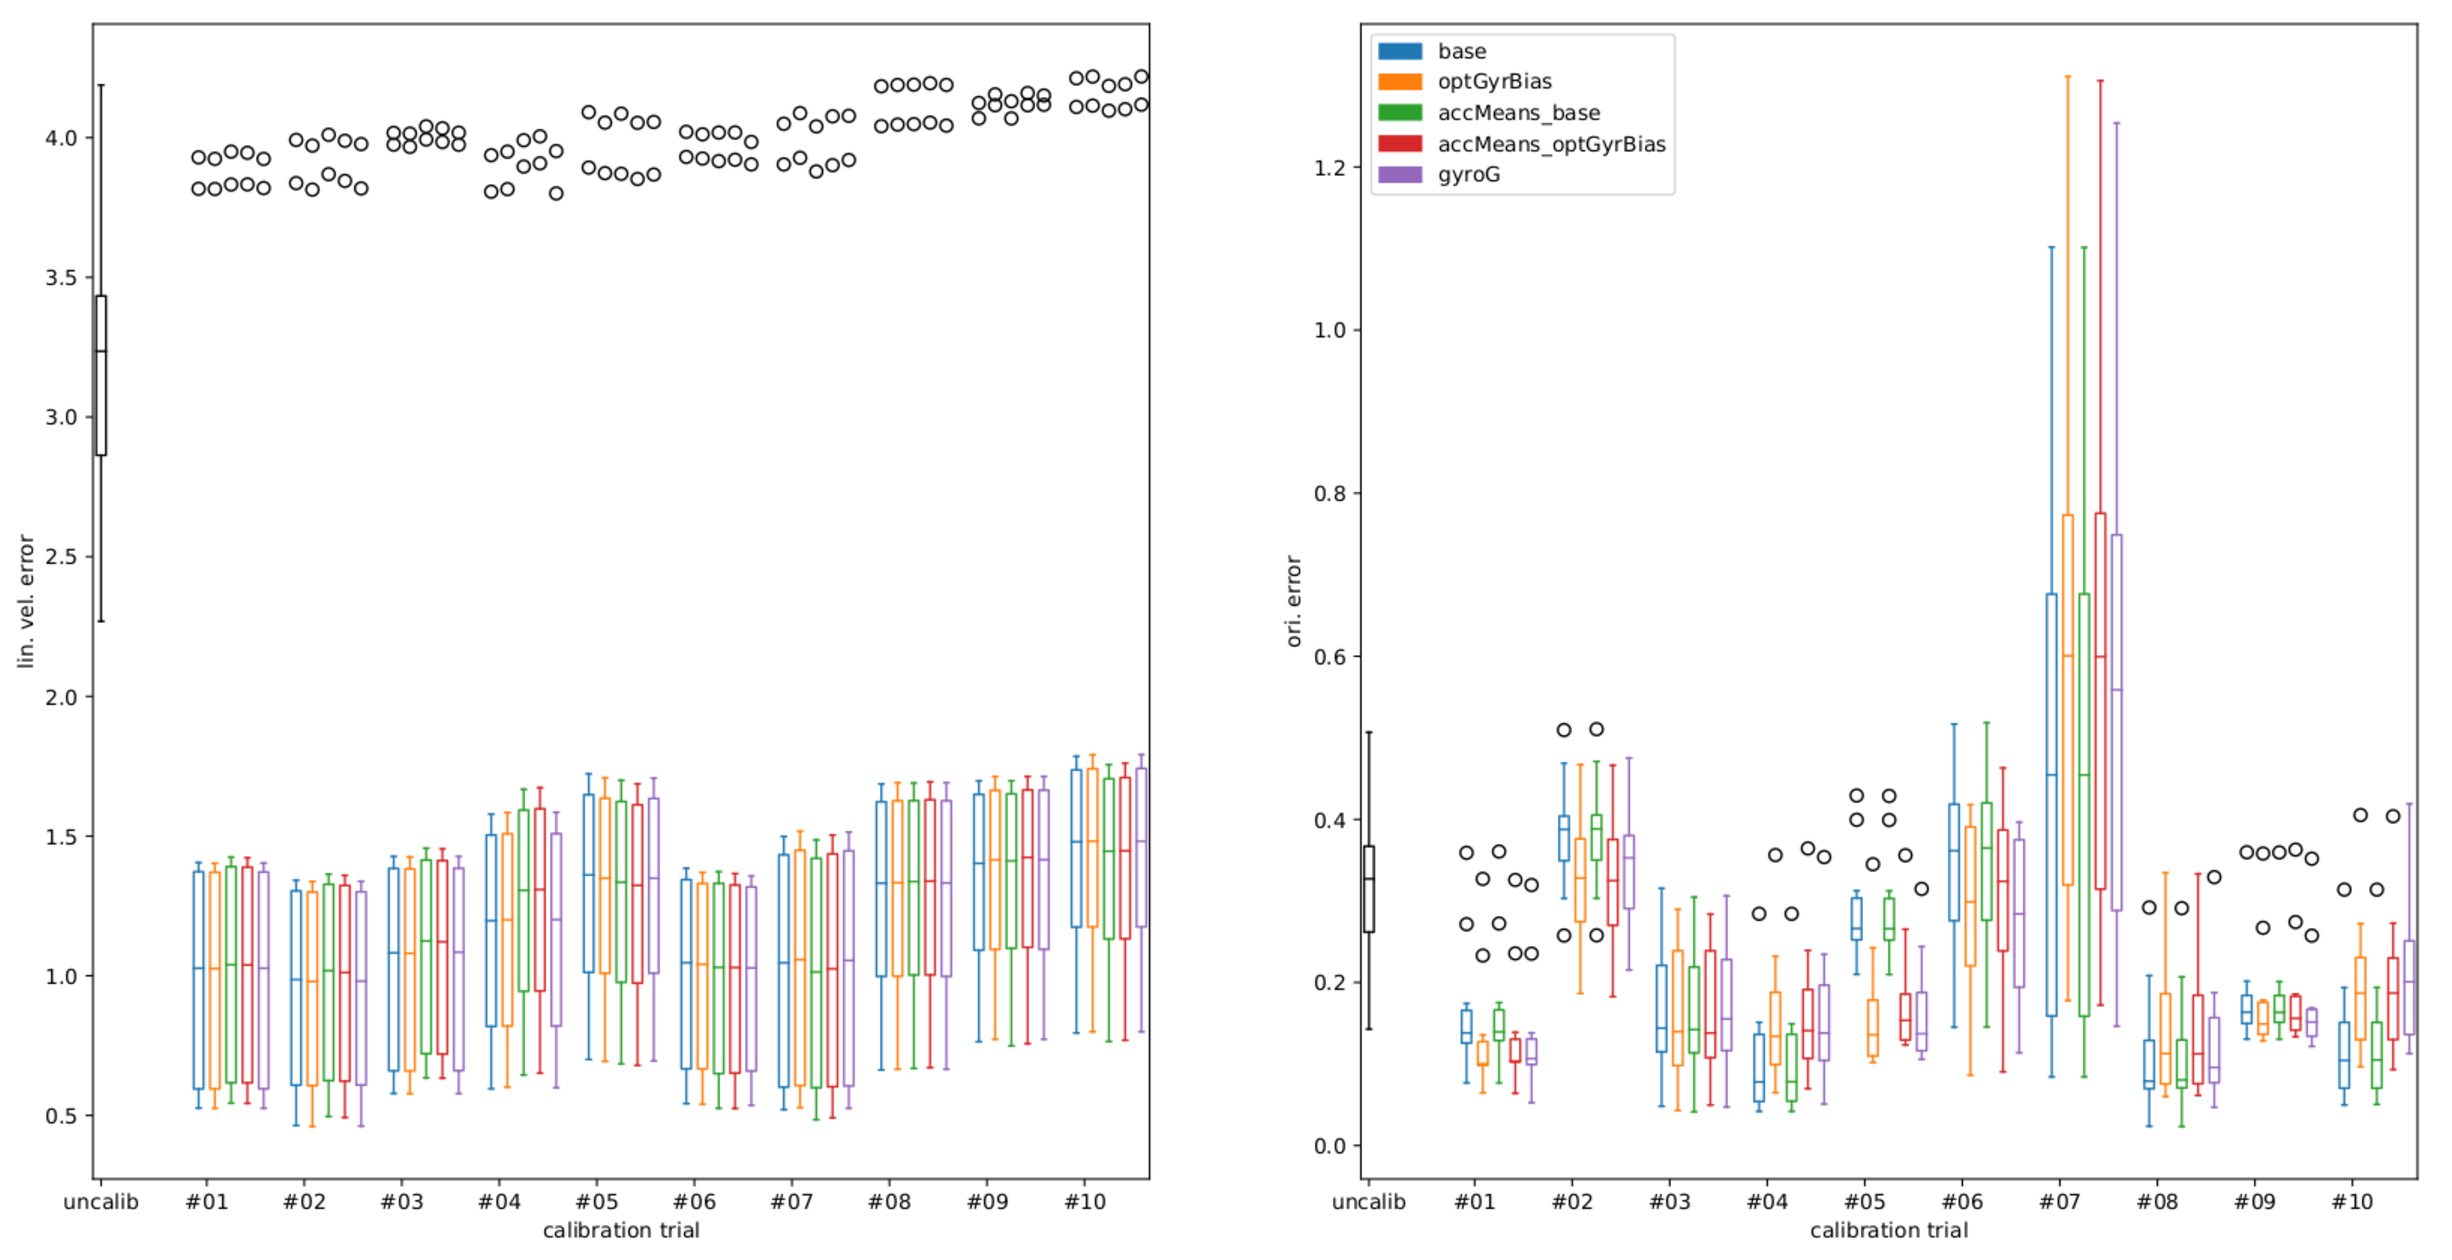
\includegraphics[width=\linewidth]{compare_calibration_trials}
	\caption{Comparison between calibrations trials. Each colour is a different combination of calibration options, black (on the left of each figure) refers to uncalibrated data. The linear velocity error (on the right) and the orientation (on the left) are calculated through the integration of the IMU readings.}
	\label{fig:comparecalibrationtrials}
\end{figure}

Figure \ref{fig:comparecalibrationmodes} compares different combinations of the calibration options, showing that the developed \texttt{opt\_gyr\_b} and \texttt{use\_gyr\_G} options slightly improve the integration error results. 

\begin{figure}[h]
	\centering
	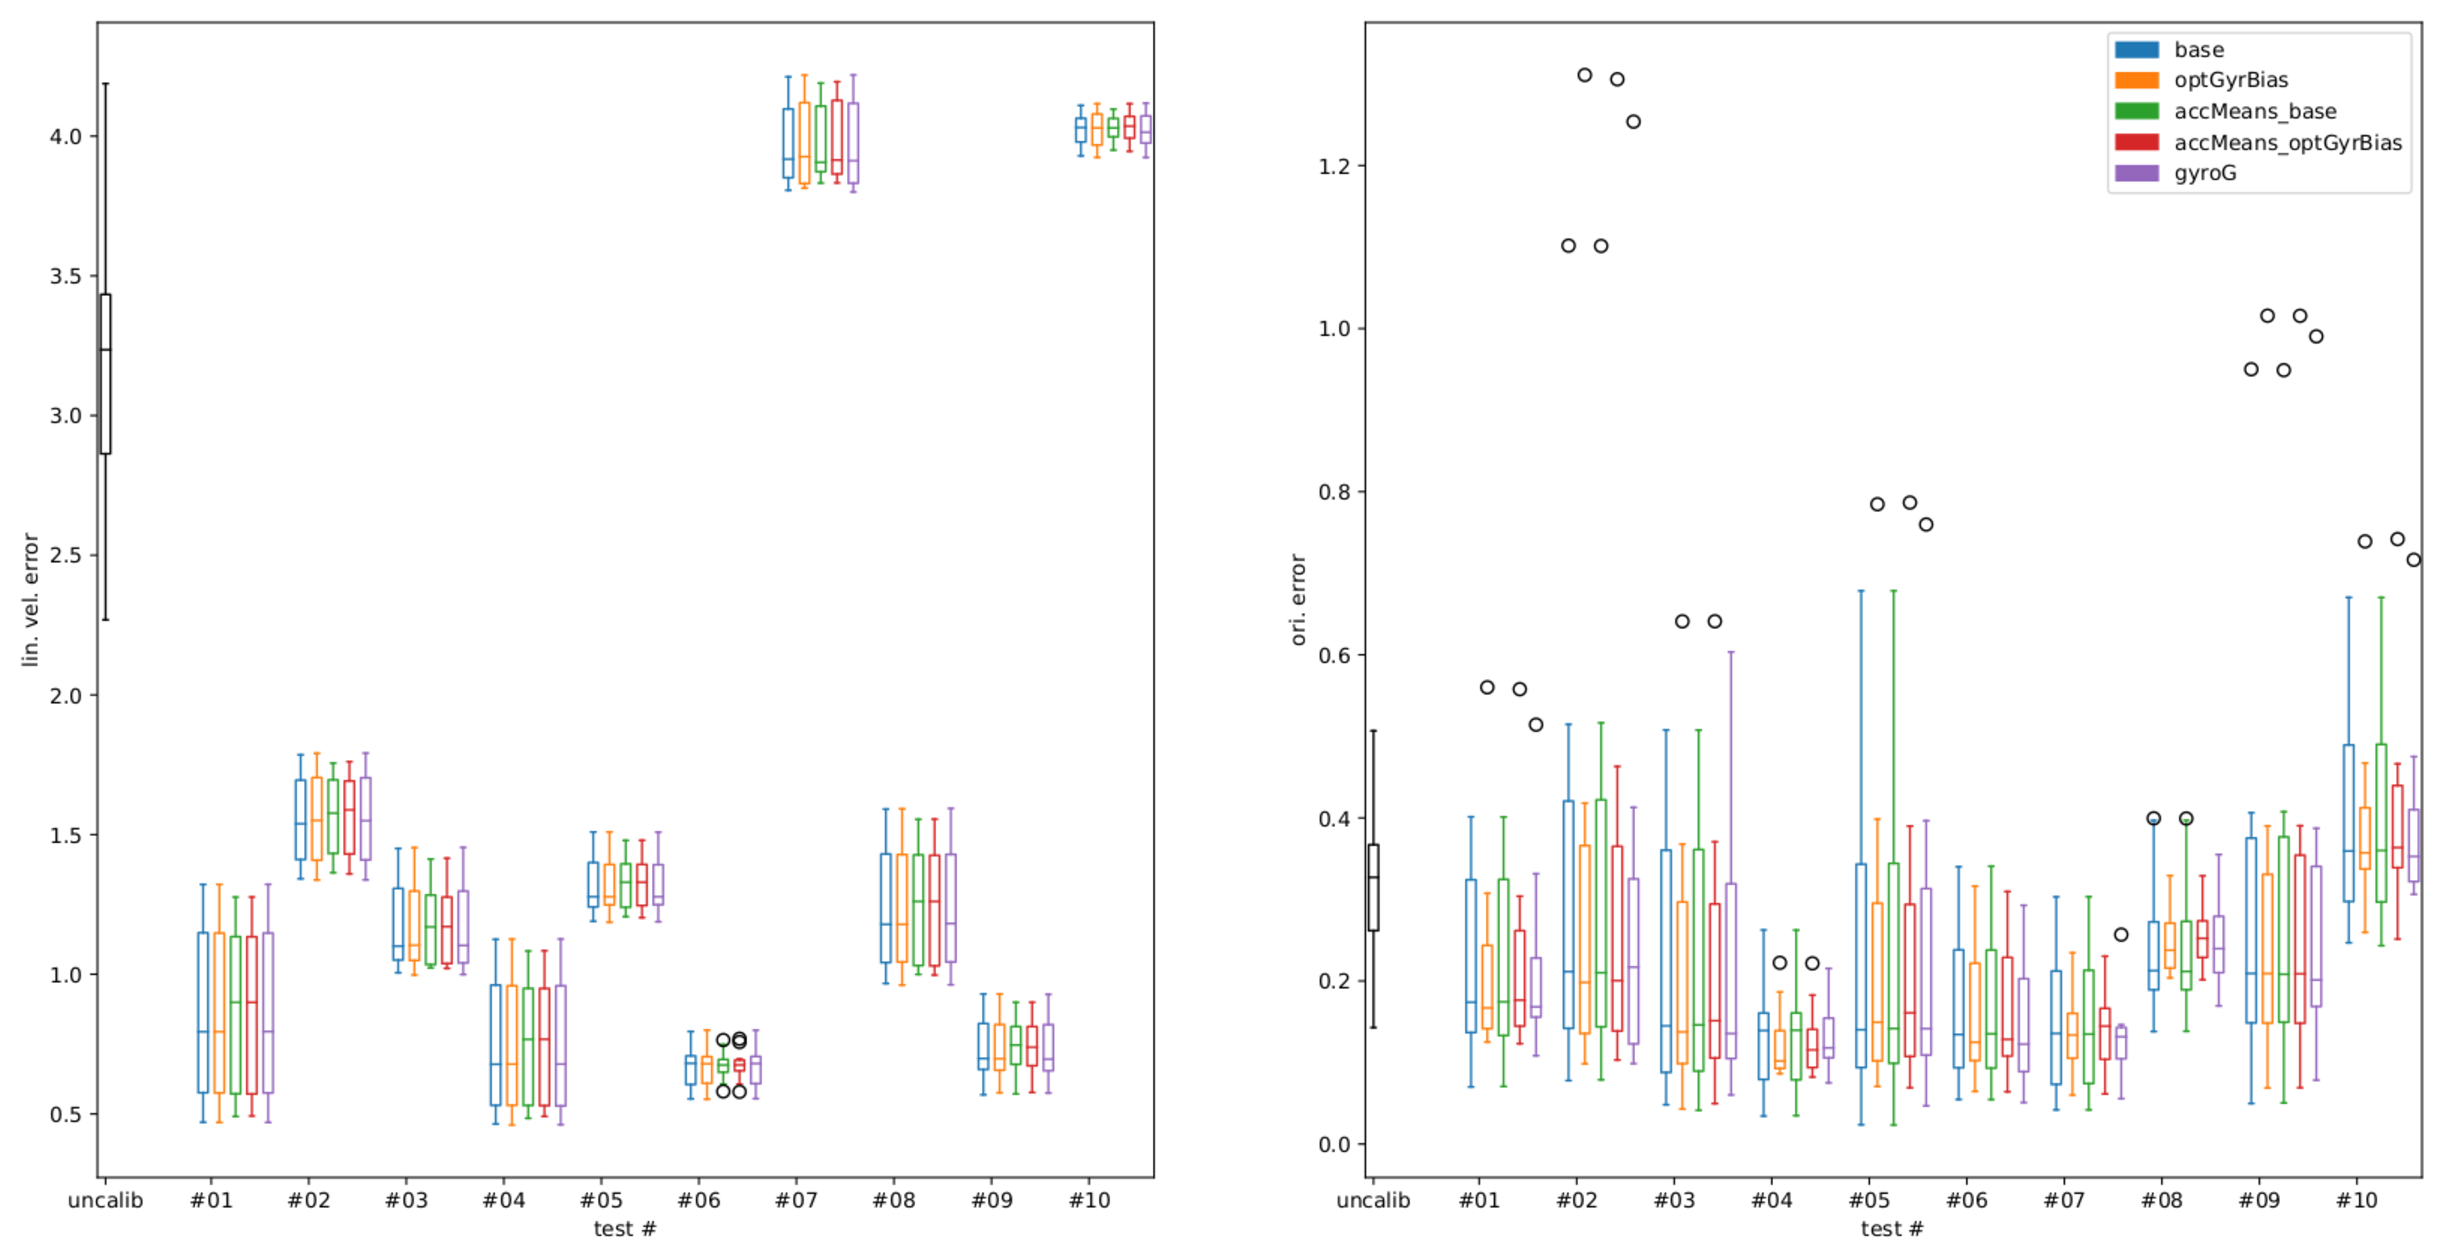
\includegraphics[width=\linewidth]{compare_calibration_modes}
	\caption{Comparison between calibration options.  Each colour is a different combination of calibration options, black (on the left of each figure) refers to uncalibrated data. The linear velocity error (on the right) and the orientation (on the left) are calculated through the integration of the IMU readings.}
	\label{fig:comparecalibrationmodes}
\end{figure}

From these tests, we conclude that more investigation can be done on the accelerometer calibration in order to pin-point what is causing the large integration error depending on the data.

Furthermore, it is worthy to remember that the accelerometer calibration impacts the gyroscope one, and the gyroscope data is used in the gravity compensation step to before integrating the linear velocities, making errors in the gyroscope calibration to propagate the other way around to the accelerometer-related results.